% !TeX encoding = UTF-8
% !TeX spellcheck = de_DE

\documentclass[biblatex]{lni}
\addbibresource{lni-paper-example-de.bib}


\usepackage{booktabs} % Schöne Tabellen mittels \toprule, \midrule, \bottomrule
\usepackage[]{blindtext} % Zu Demonstrationszwecken
\usepackage{fancyhdr}
\usepackage{acronym}

%% Sietenzahlen
\pagestyle{fancy}
\fancyhf{}
\fancyfoot[C]{\thepage}
\renewcommand{\headrulewidth}{0pt}

\begin{document}

\begin{titlepage}
  \centering
  \vspace*{0.5cm}

  {\scshape\LARGE Fallstudie \par}

  {\huge\bfseries
    Analyse von Web Applikations-Technologien:
  \par
  }
  {\Large\itshape Am Beispiel der Planung einer GLS Quiz App\par}

  \vspace{1cm}

  {\Large\textbf{Eingereicht von: }}\\
  Nicolas Fritz \\
  E-Mail: nicolasnoah.fritz@gls-germany.com

  \vspace{1cm}

  {\Large\textbf{Eingereicht bei: }}\\
  Hochschule Fulda \\
  Leipziger Straße 123 \\
  36037 Fulda \\
  Lehrperson: Prof. Dr. Brigit Bomsdorf

  \vspace{1cm}

  {\Large\textbf{Unternehmen: }}\\
  GLS Germany GmbH & Co. OHG \\
  Betreuung: Laura Alles, Patrick Weppler

  \vfill

  {\large \today\par}
\end{titlepage}

\tableofcontents
\listoffigures
\newpage

\section*{Abkürzungsverzeichnis}
\begin{acronym}[Bash]
  \acro{HTML}{Hypertext Markup Language}
  \acro{CSS}{Cascading Style Sheets}
  \acro{JS}{JavaScript}
\end{acronym}
\newpage

\section{Einleitung}
Diese Fallstudie mit dem Titel „Analyse von Web Applikations-Technologien: Am Beispiel der Planung einer GLS Quiz App“
wurde im Fachbereich Angewandte Informatik von Nicolas Fritz im Unternehmen GLS Germany GmbH & Co. OHG erstellt.
Die Betreuung im Unternehmen erfolgte durch Patrick Weppler für den technischen Teil und Laura Alles für den konzeptionellen Teil.
An der Hochschule wurde die Arbeit von Prof. Dr. Birgit Bomsdorf betreut.
Das Thema wird anhand des Fallbeispiels einer GLS Quiz App erläutert und analysiert.

\subsection{Hintergrund und Motivation}
Software wird zunehmend komplexer und enthält immer mehr Funktionen, von denen viele standardisiert und wiederkehrend sind.
Je größer das Projekt, desto schwieriger wird es, den Überblick zu behalten – insbesondere bei Webanwendungen,
die sich kontinuierlich weiterentwickeln und fortlaufend programmiert werden.
Um den Überblick zu bewahren, sind daher Konzepte notwendig, die eine Erweiterbarkeit sicherstellen.
Außerdem muss Software skalierbar und gleichzeitig effizient sein.

\\

Ein Beispiel für eine solche Webanwendung ist die GLS-Quiz App.
Diese App dient dazu, neue duale Studenten, Auszubildende oder Mitarbeiter mit dem Unternehmen vertraut zu machen.
Sie basiert auf einer zuvor genutzten analogen Version, in der die Nutzer in die Rolle eines Paketboten schlüpfen,
Pakete ausliefern und dabei auf verschiedene Probleme stoßen, die sie durch das Beantworten von Fragen lösen müssen.

\\

Im Verlauf der Konzeptionierung und Umsetzung der App stellte sich heraus,
dass die ursprüngliche analoge Version aufgrund der gewählten Technologie stark vereinfacht werden musste
und die Weiterentwicklung nun deutlich erschwert ist.

\\

Daher benötigen wir eine Lösung,
die eine vorgegebene Struktur bietet und grundlegende Funktionen bereits integriert.
Gleichzeitig müssen einfache Erweiterungsmöglichkeiten gewährleistet sein.

\subsection{Ziel der Fallstudie}

\subsection{Methodik und Vorgehensweise}

\section{Technologieüberblick}
\Cref{fig:eftFramework} zeigt eine Abbildung.
\begin{figure}
  \centering
  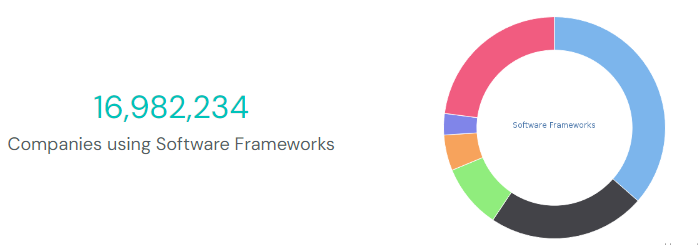
\includegraphics[width=.8\textwidth]{eftFramework}
  \caption{Frameworknutzung bei Unternehmen.}
  \label{fig:eftFramework}
  \vspace{-0.3cm}
  \begin{center}
    \footnotesize Quelle: \cite{eftFramework}
  \end{center}
\end{figure}

\subsection{Überblick über moderne Webtechnologien}
\subsection{Frontend-Technologien im Vergleich: VueJS, Angular und React}
\Cref{fig:fetrends} zeigt eine Abbildung.

\begin{figure}
  \centering
  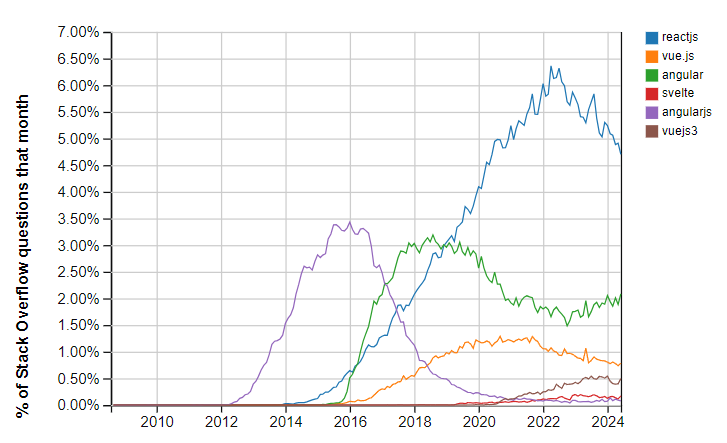
\includegraphics[width=.8\textwidth]{fetrends}
  \caption{Stackoverflow Fragen Frontend-Frameworks.}
  \label{fig:fetrends}
  \vspace{-0.3cm}
  \begin{center}
    \footnotesize Quelle: \cite{SOTrend}
  \end{center}
\end{figure}

\subsection{Backend-Technologien im Vergleich: Express, Springboot und Django}
\subsection{Wie arbeiten Backend und Frontend zusammen?}

\section{Die GLS Quiz App}
\subsection{Ist-Zustand der App}
\subsection{Ursprüngliches Konzept}
\subsection{Probleme bei der Umsetzbarkeit des ursprünglichen Konzepts}
\subsection{Konzeptentwicklung zur Bewältigung der Herausforderungen}

\section{Test-Implementierung}
\subsection{Das Demo Projekt}
\subsection{Umsetzung}
\subsection{Ergebnisse und erlangtes Wissen}

\section{Schlussfolgerung und Ausblick}

\newpage
\printbibliography

\end{document}
